%%%%%%%%%%%%%%%%%%%%%%%%%%%%%%%%%%%%%%%%%
% baposter Landscape Poster
% LaTeX Template
% Version 1.0 (11/06/13)
%
% baposter Class Created by:
% Brian Amberg (baposter@brian-amberg.de)
%
% This template has been downloaded from:
% http://www.LaTeXTemplates.com
%
% License:
% CC BY-NC-SA 3.0 (http://creativecommons.org/licenses/by-nc-sa/3.0/)
%
%%%%%%%%%%%%%%%%%%%%%%%%%%%%%%%%%%%%%%%%%

%----------------------------------------------------------------------------------------
%	PACKAGES AND OTHER DOCUMENT CONFIGURATIONS
%----------------------------------------------------------------------------------------

\documentclass[landscape,a0paper,fontscale=0.290]{baposter} % Adjust the font scale/size here

\usepackage{graphicx} % Required for including images
\graphicspath{{figures/}} % Directory in which figures are stored

\usepackage{amsmath} % For typesetting math
\usepackage{amssymb} % Adds new symbols to be used in math mode

\usepackage{booktabs} % Top and bottom rules for tables
\usepackage{enumitem} % Used to reduce itemize/enumerate spacing
\usepackage{palatino} % Use the Palatino font
\usepackage[font=small,labelfont=bf]{caption} % Required for specifying captions to tables and figures

\usepackage{multicol} % Required for multiple columns
\setlength{\columnsep}{1.5em} % Slightly increase the space between columns
\setlength{\columnseprule}{0mm} % No horizontal rule between columns

\usepackage{tikz} % Required for flow chart
\usetikzlibrary{shapes,arrows} % Tikz libraries required for the flow chart in the template

\newcommand{\compresslist}{ % Define a command to reduce spacing within itemize/enumerate environments, this is used right after \begin{itemize} or \begin{enumerate}
\setlength{\itemsep}{1pt}
\setlength{\parskip}{0pt}
\setlength{\parsep}{0pt}
}

\definecolor{lightblue}{rgb}{0.145,0.6666,1} % Defines the color used for content box headers

\begin{document}

\begin{poster}
{
headerborder=closed, % Adds a border around the header of content boxes
colspacing=1em, % Column spacing
bgColorOne=white, % Background color for the gradient on the left side of the poster
bgColorTwo=white, % Background color for the gradient on the right side of the poster
borderColor=lightblue, % Border color
headerColorOne=black, % Background color for the header in the content boxes (left side)
headerColorTwo=lightblue, % Background color for the header in the content boxes (right side)
headerFontColor=white, % Text color for the header text in the content boxes
boxColorOne=white, % Background color of the content boxes
textborder=roundedleft, % Format of the border around content boxes, can be: none, bars, coils, triangles, rectangle, rounded, roundedsmall, roundedright or faded
eyecatcher=true, % Set to false for ignoring the left logo in the title and move the title left
headerheight=0.15\textheight, % Height of the header
headershape=roundedright, % Specify the rounded corner in the content box headers, can be: rectangle, small-rounded, roundedright, roundedleft or rounded
headerfont=\Large\bf\textsc, % Large, bold and sans serif font in the headers of content boxes
%textfont={\setlength{\parindent}{1.5em}}, % Uncomment for paragraph indentation
linewidth=2pt % Width of the border lines around content boxes
}
%----------------------------------------------------------------------------------------
%	TITLE SECTION 
%----------------------------------------------------------------------------------------
%
{
\includegraphics[height=4em]{SB_Logo.png}} % First university/lab logo on the left
{\bf\textsc{Construction of a Magnetic Field Cloaking Device For Use in a Proposed Electron Ion Collider}\vspace{0.5em}} % Poster title
{\textsc{\textbf{Thomas Krahulik}, \textbf{Joshua LaBounty}, Dr. Abhay Deshpande, Dr. Nils Feege \\ Stony Brook University, Department of Physics and Astronomy \\ Brookhaven National Laboratory $\bullet$ Argonne Nation al Laboratory}}% Author names and institution
{\hspace{10mm} 
\includegraphics[height=8em]{CreatedEICLogo.png}} % Second university/lab logo on the right

%----------------------------------------------------------------------------------------
%	Electron Ion Collider
%----------------------------------------------------------------------------------------

\headerbox{Background}{name=EIC,column=0,row=0}{

The current design for a proposed Electron Ion Collider (EIC) calls for a hadron to electron beam momentum ratio of 12:1, resulting in a large number of particles produced in the forward region. Employing a substantial magnetic field orthogonal to the beam line is optimal for momentum analysis of such particles, but the collider beams must be shielded from the orthogonal field to avoid beam deflection and depolarization. Here, we demonstrate the potential of a magnetic field cloaking device to passively create a field free tunnel while minimizing distortions of the applied external field

}

%----------------------------------------------------------------------------------------
%	DIS Physics
%----------------------------------------------------------------------------------------

%\headerbox{Pythia Simulation}{name=method,column=0,below=objectives,bottomaligned=conclusion}{ % This block's bottom aligns with the bottom of the conclusion block
\headerbox{Cloak Construction}{name=method,column=0,below=EIC,above=bottom}{

%\begin{multicols}{2}

%\begin{center}
%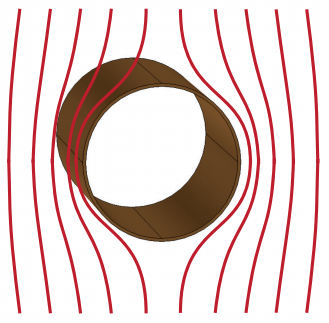
\includegraphics[width=0.97\linewidth]{ShieldConcept.png}
%\captionof{figure}{Superconductors expel magnetic fields through the Meissner effect.}
%\end{center}

%\begin{center}
%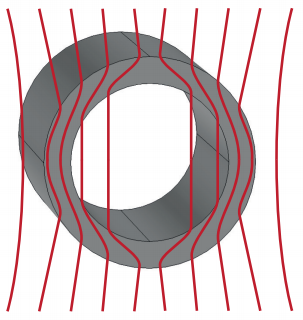
\includegraphics[width=0.92\linewidth]{Ferromagnet-Concept.png}
%\captionof{figure}{Ferromagnet Theory}
%\end{center}

%\end{multicols}

A superconductor naturally expels magnetic field lines through the Meissner effect, while a ferromagnet pulls them in. By combining the two effects, you can achieve a field free region in the center while keeping the outside field undisturbed.

\begin{center}
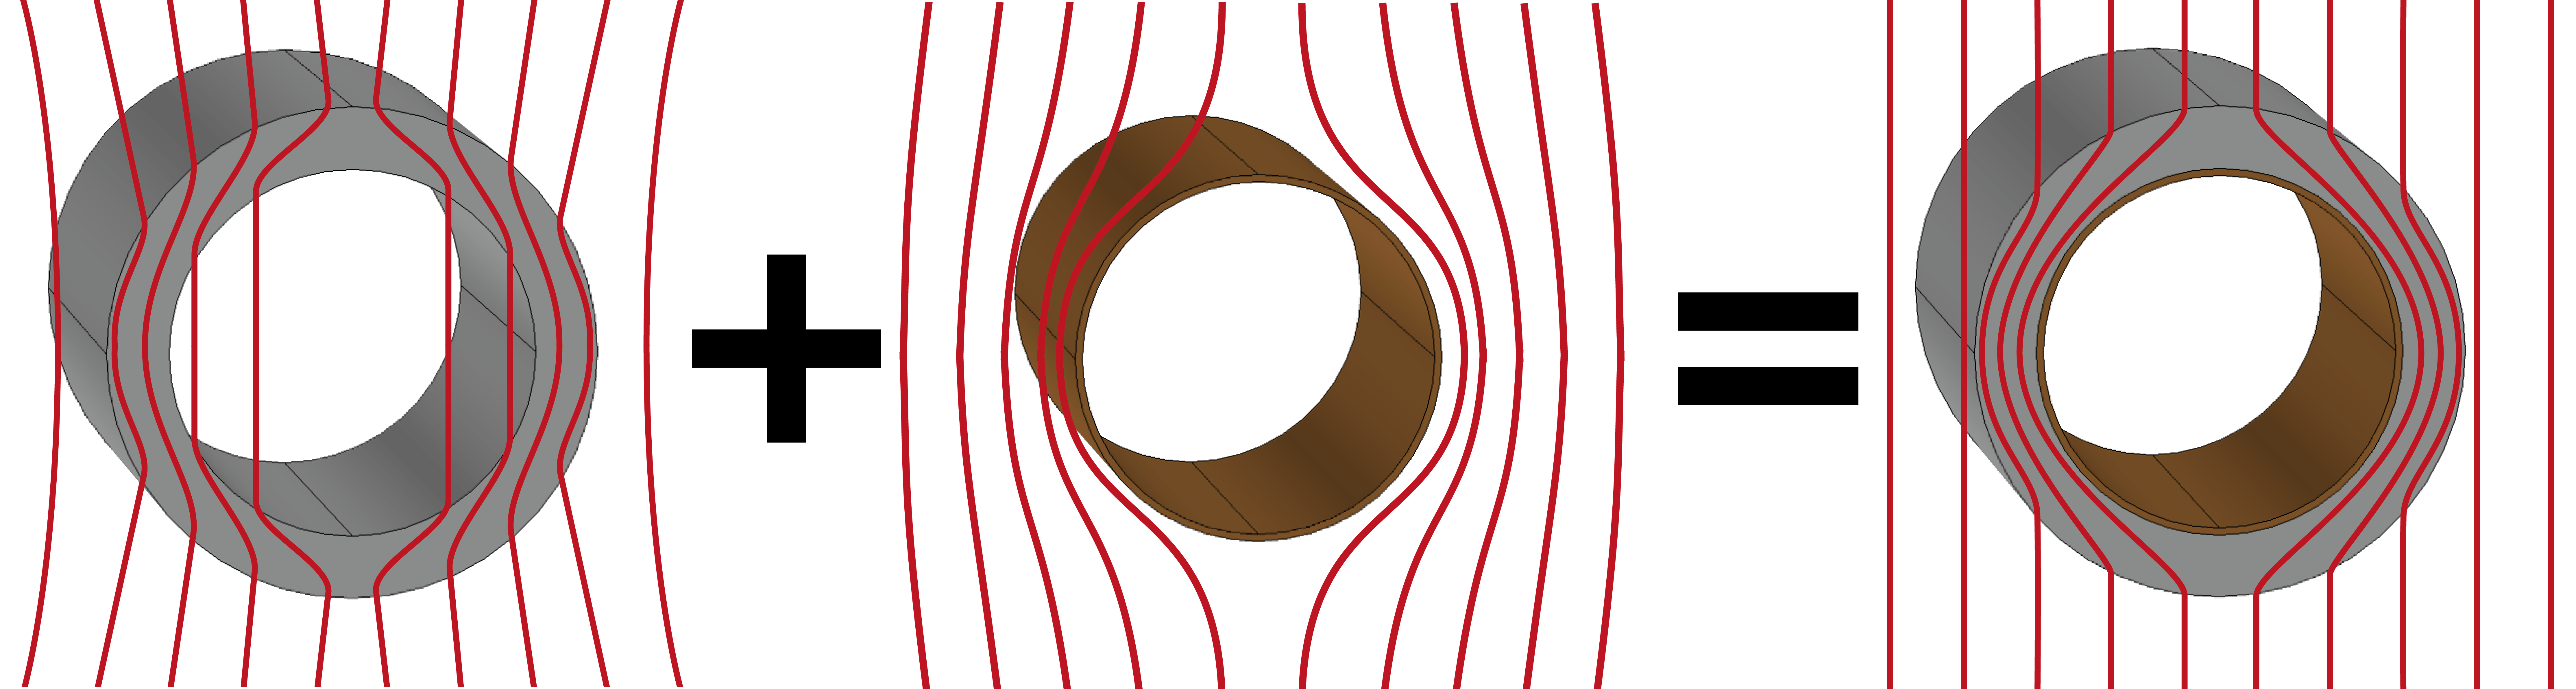
\includegraphics[width=\linewidth]{SC_plus_FM_equals_Cloak.png}
\captionof{figure}{Our magnetic cloak is composed of two concentric cylinders: one made of superconductor and one made of a ferromagnet/epoxy mixture.}
\end{center}

We demonstrate the feasibility of this cloak using 45-layers of YBCO superconductor surrounded by a carefully tuned epoxy/ferromagnet mixture.

\begin{center}
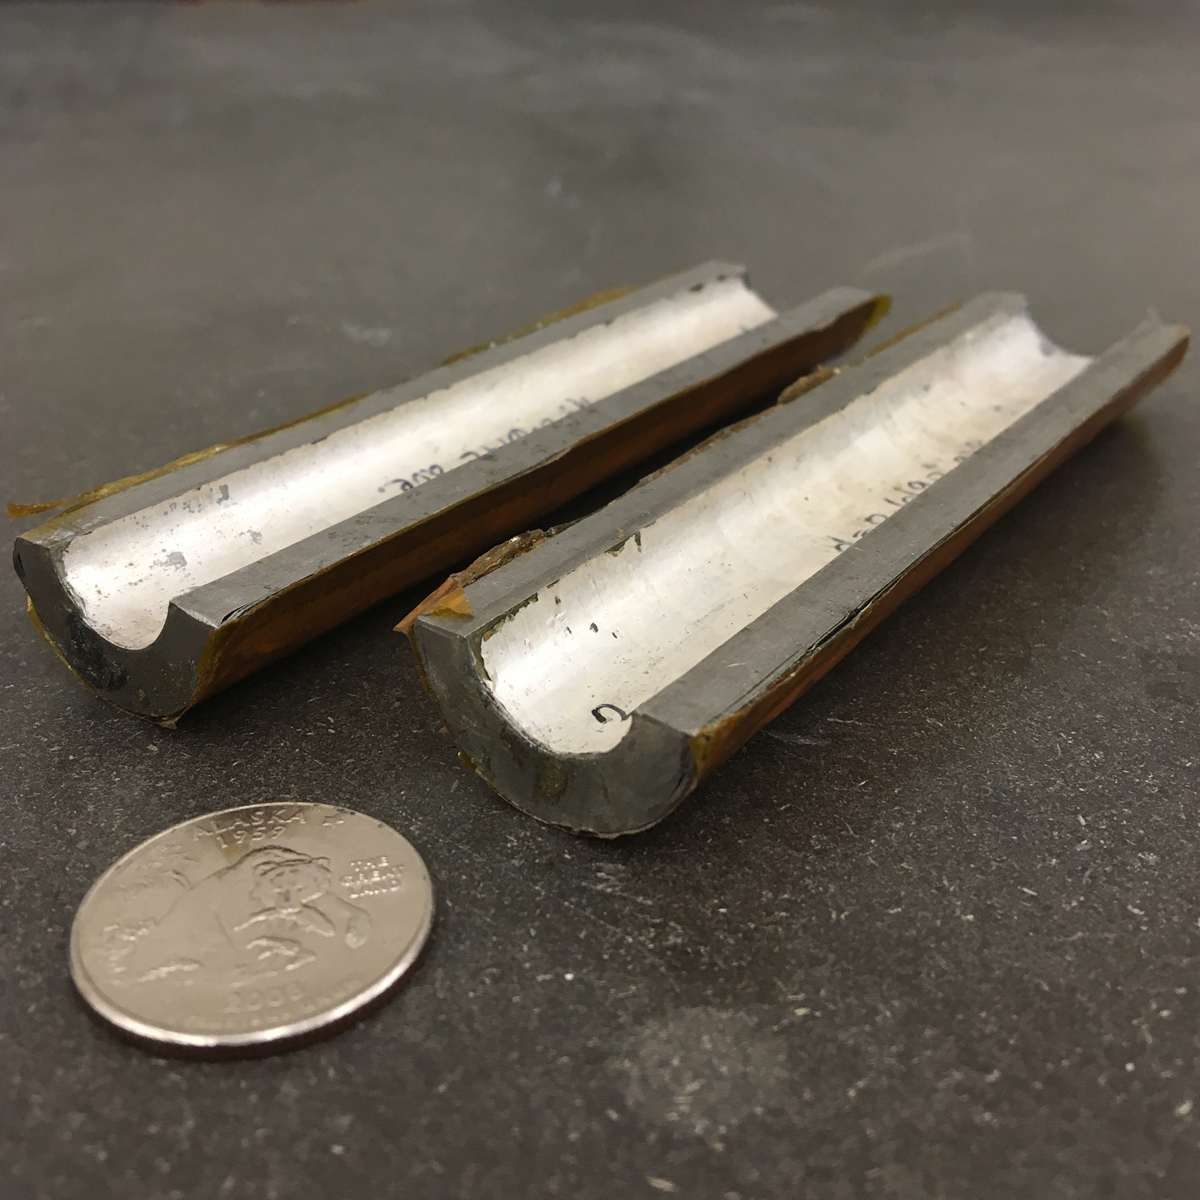
\includegraphics[width=0.46\linewidth]{pic_sc45layer.jpg}
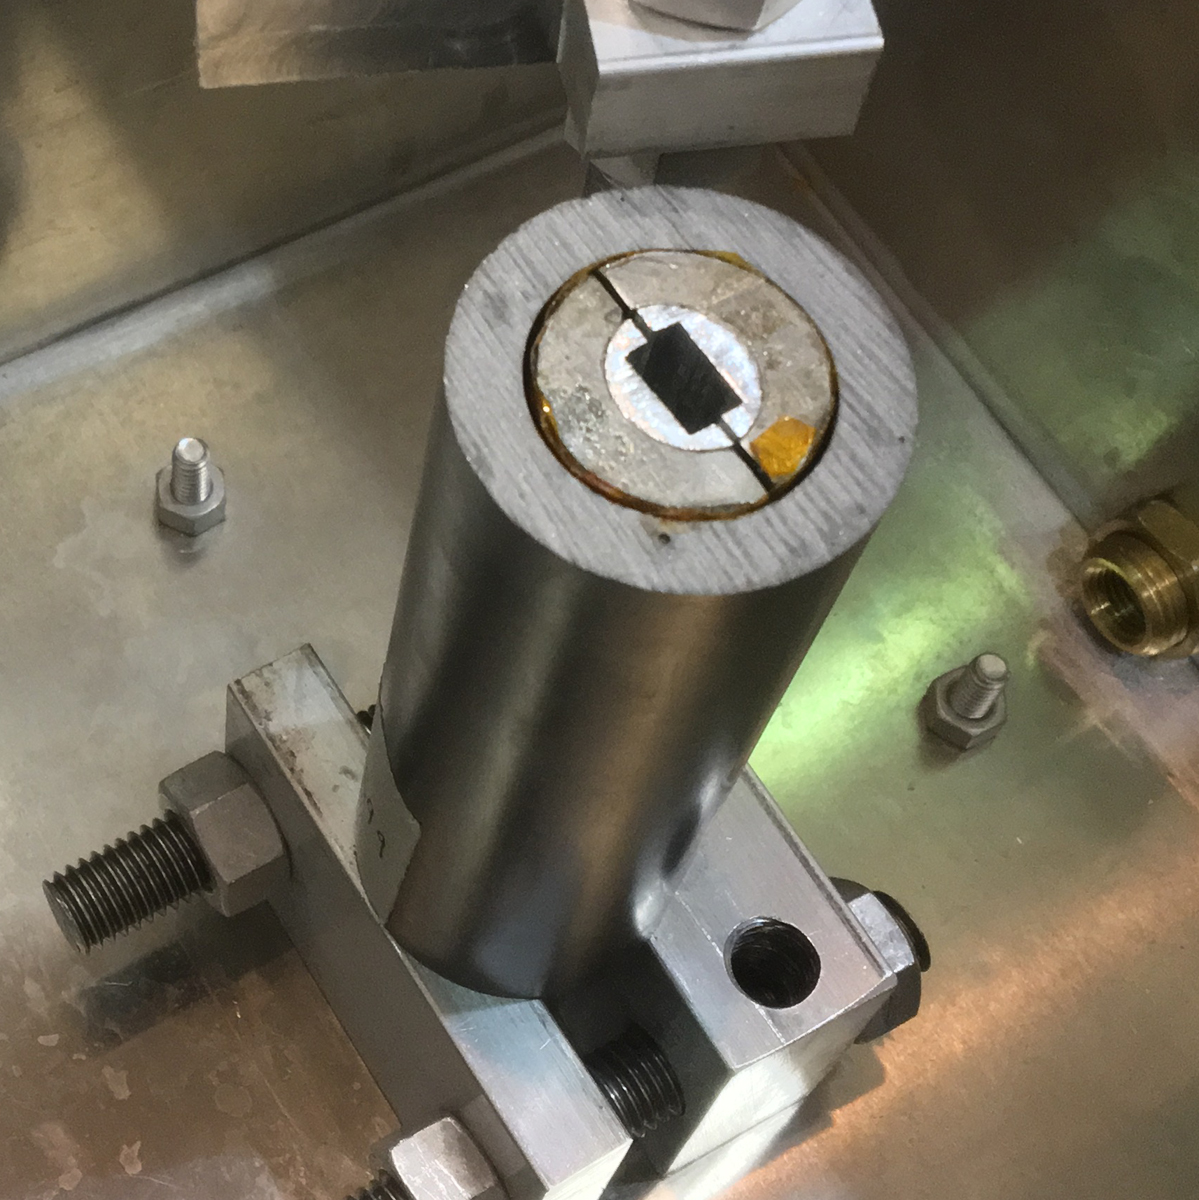
\includegraphics[width=0.46\linewidth]{pic_cloak.jpg}
\captionof{figure}{Images of our 45-layer cloak prototype.}
\end{center}

}

%----------------------------------------------------------------------------------------
%	Pythia Simulation
%----------------------------------------------------------------------------------------

\headerbox{Superconductor Shielding}{name=introduction,column=1,span=2,row=0}{
\begin{multicols}{3}
\begin{center}
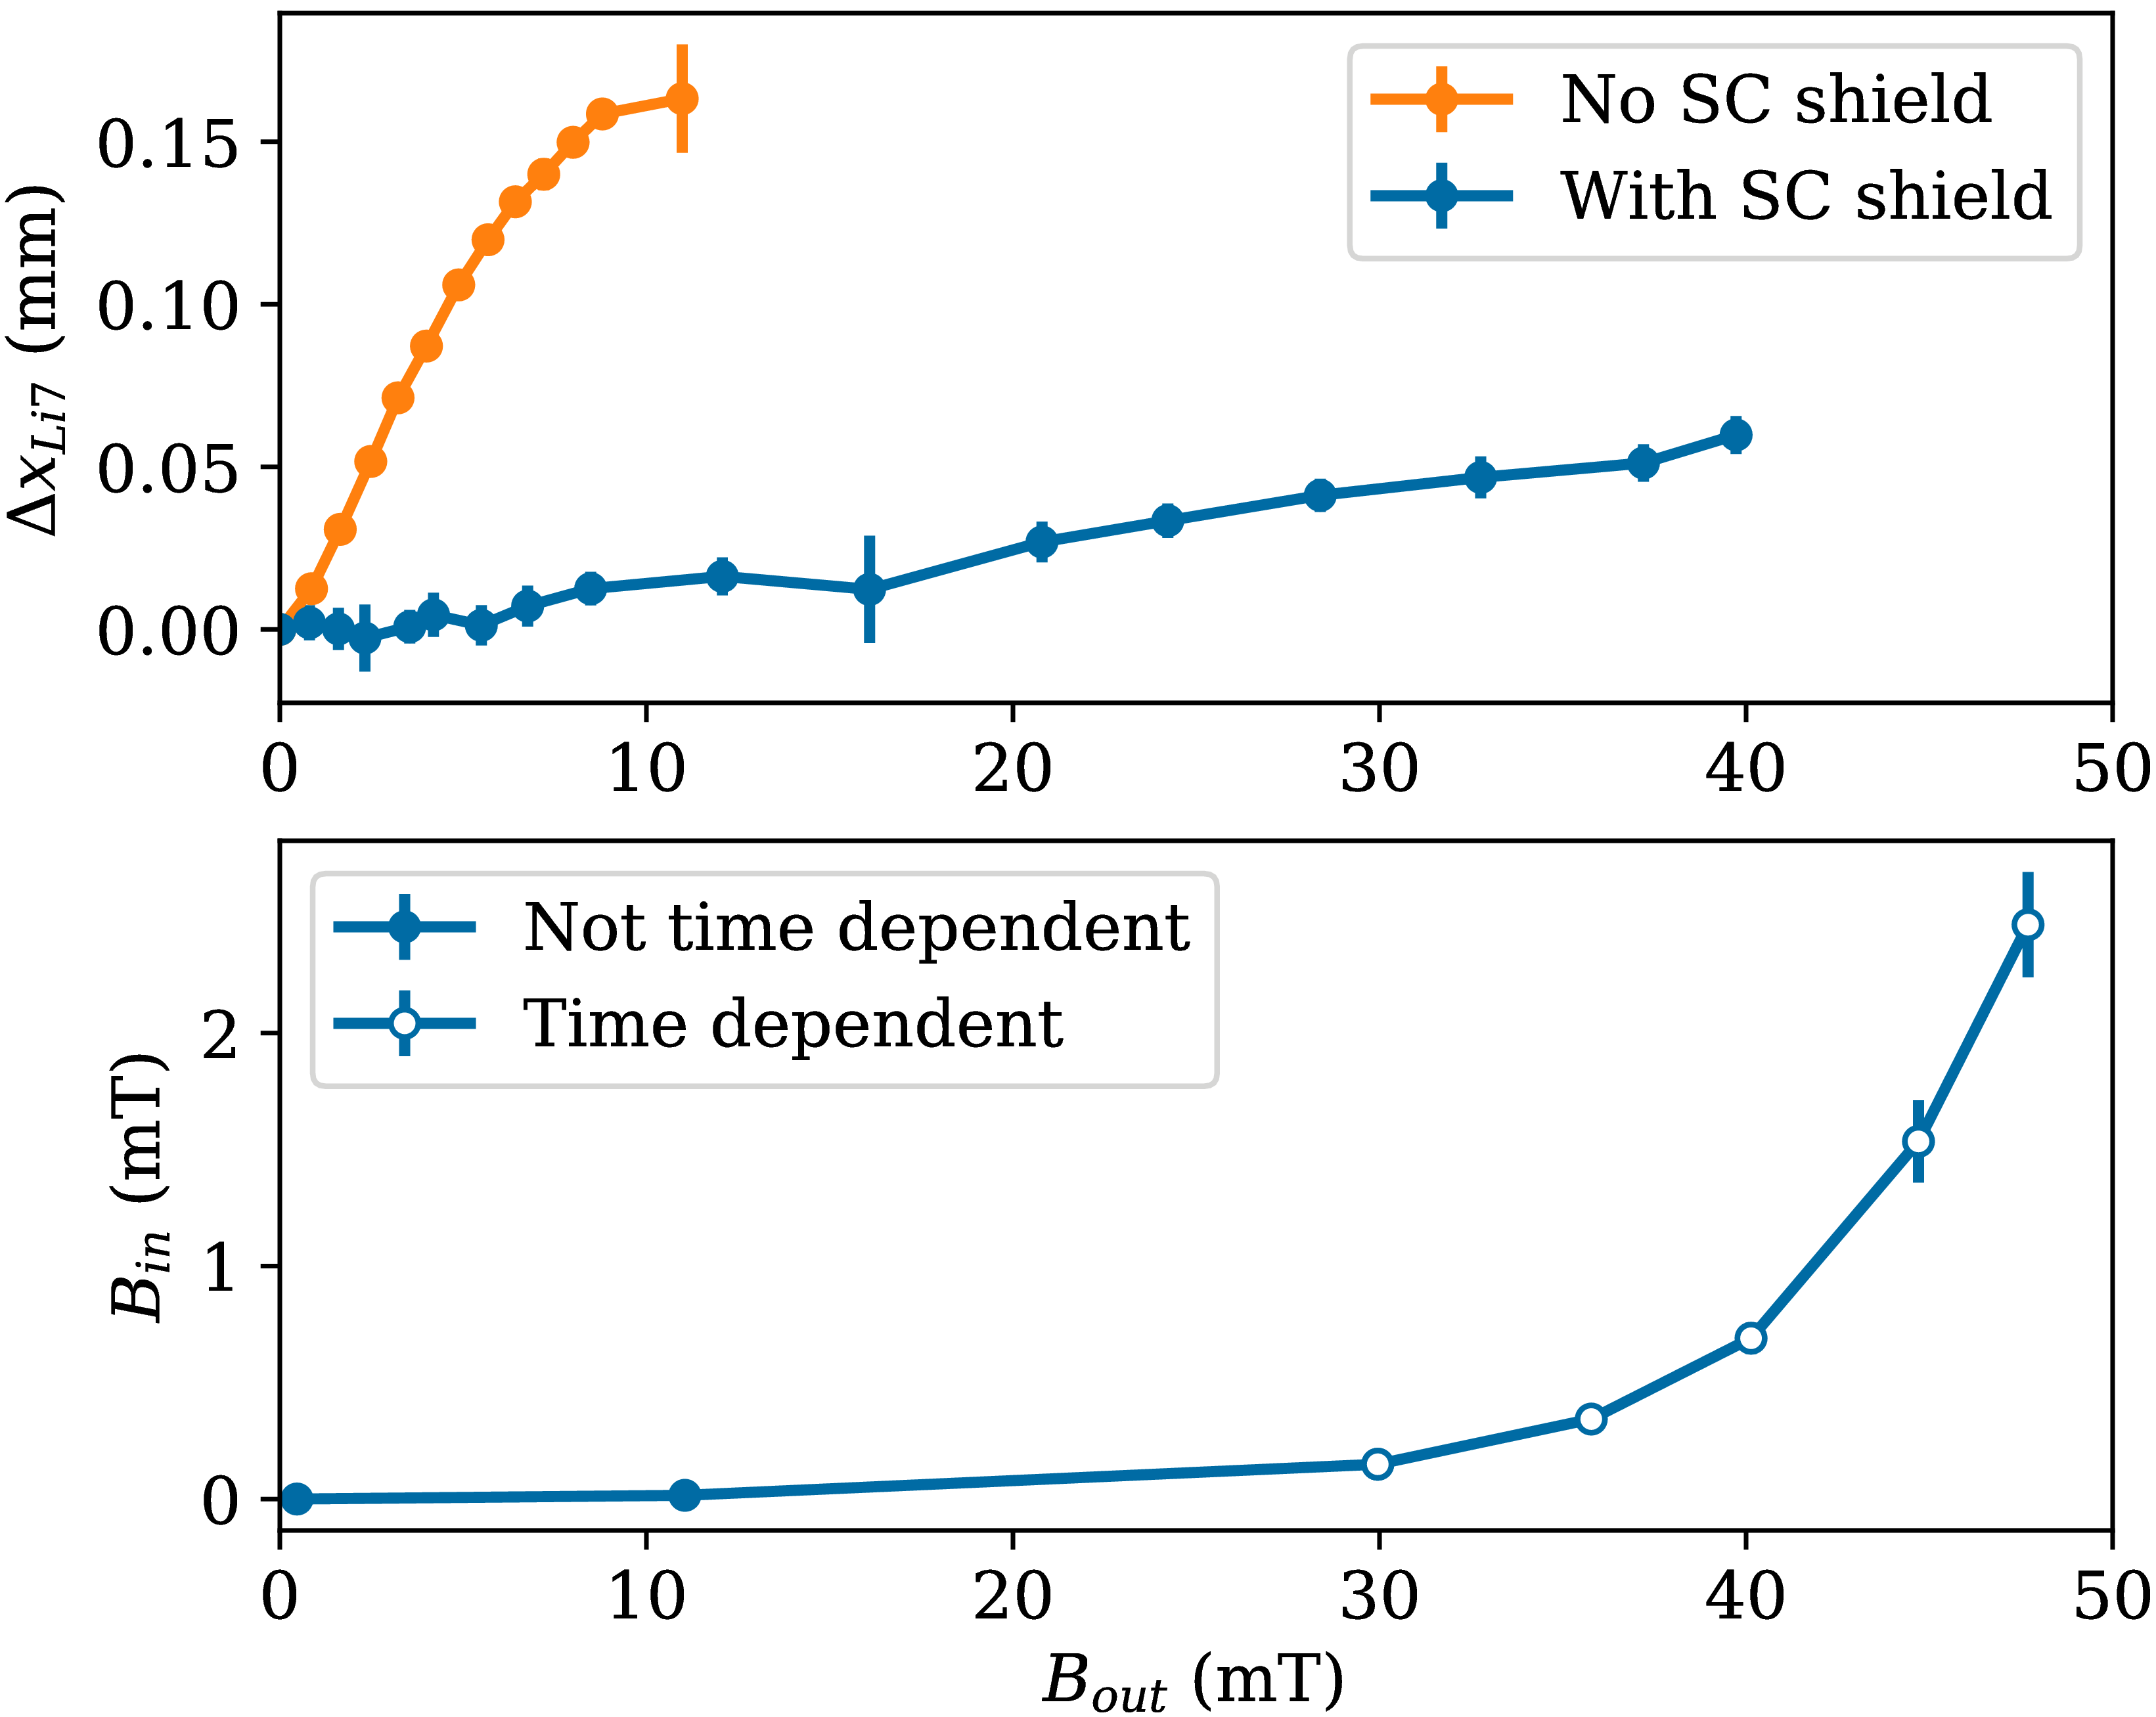
\includegraphics[width=1.0\linewidth]{shielding_vdg2layer.png}
\captionof{figure}{Measurement of shielding of the 2-layer, 1-meter prototype at SBU and BNL using both Hall Probes and the deflection of a Lithium-7 beam.}
\end{center}
\begin{center}
\hspace*{-1.5em} 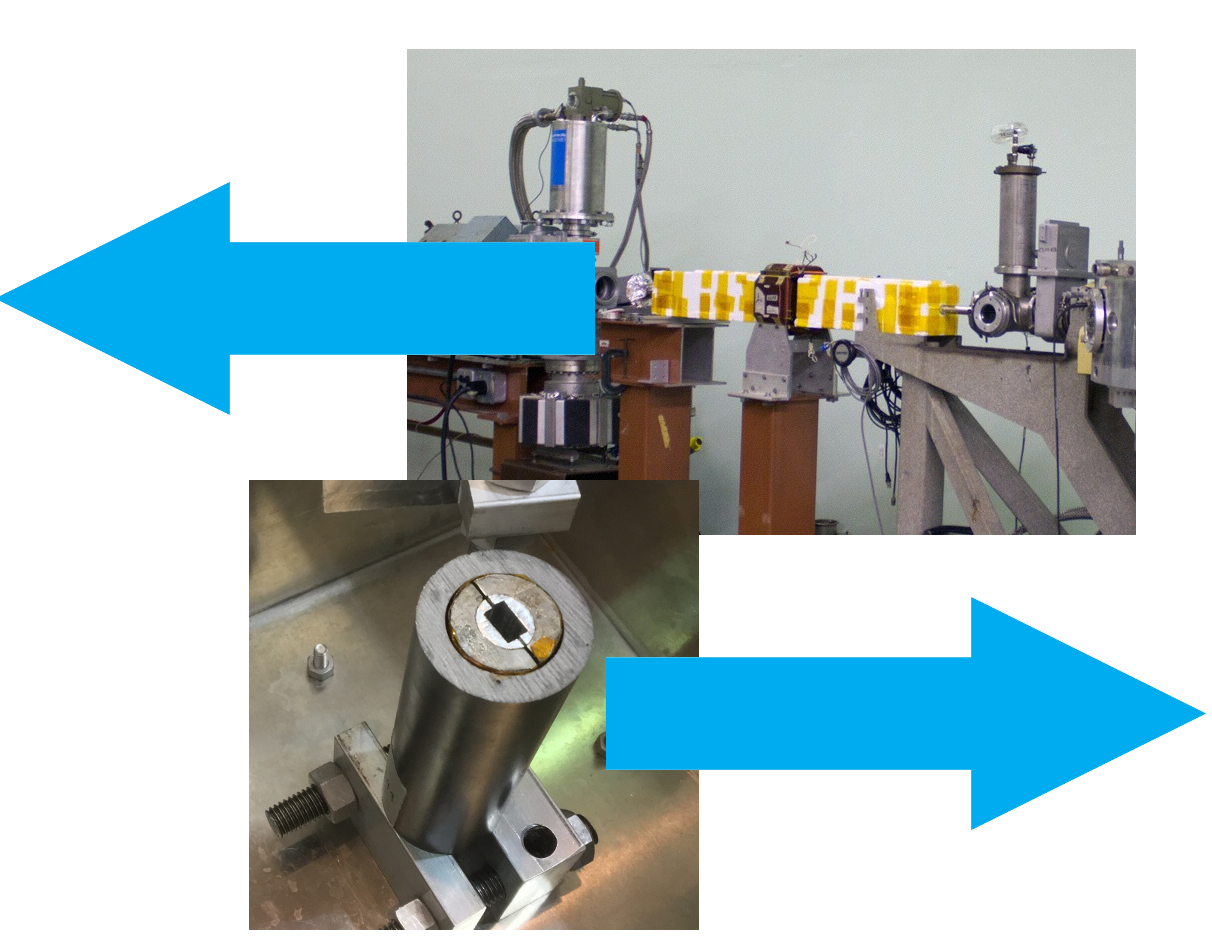
\includegraphics[width=1.2\linewidth]{Setup_Diagram.png}
\end{center}
\begin{center}
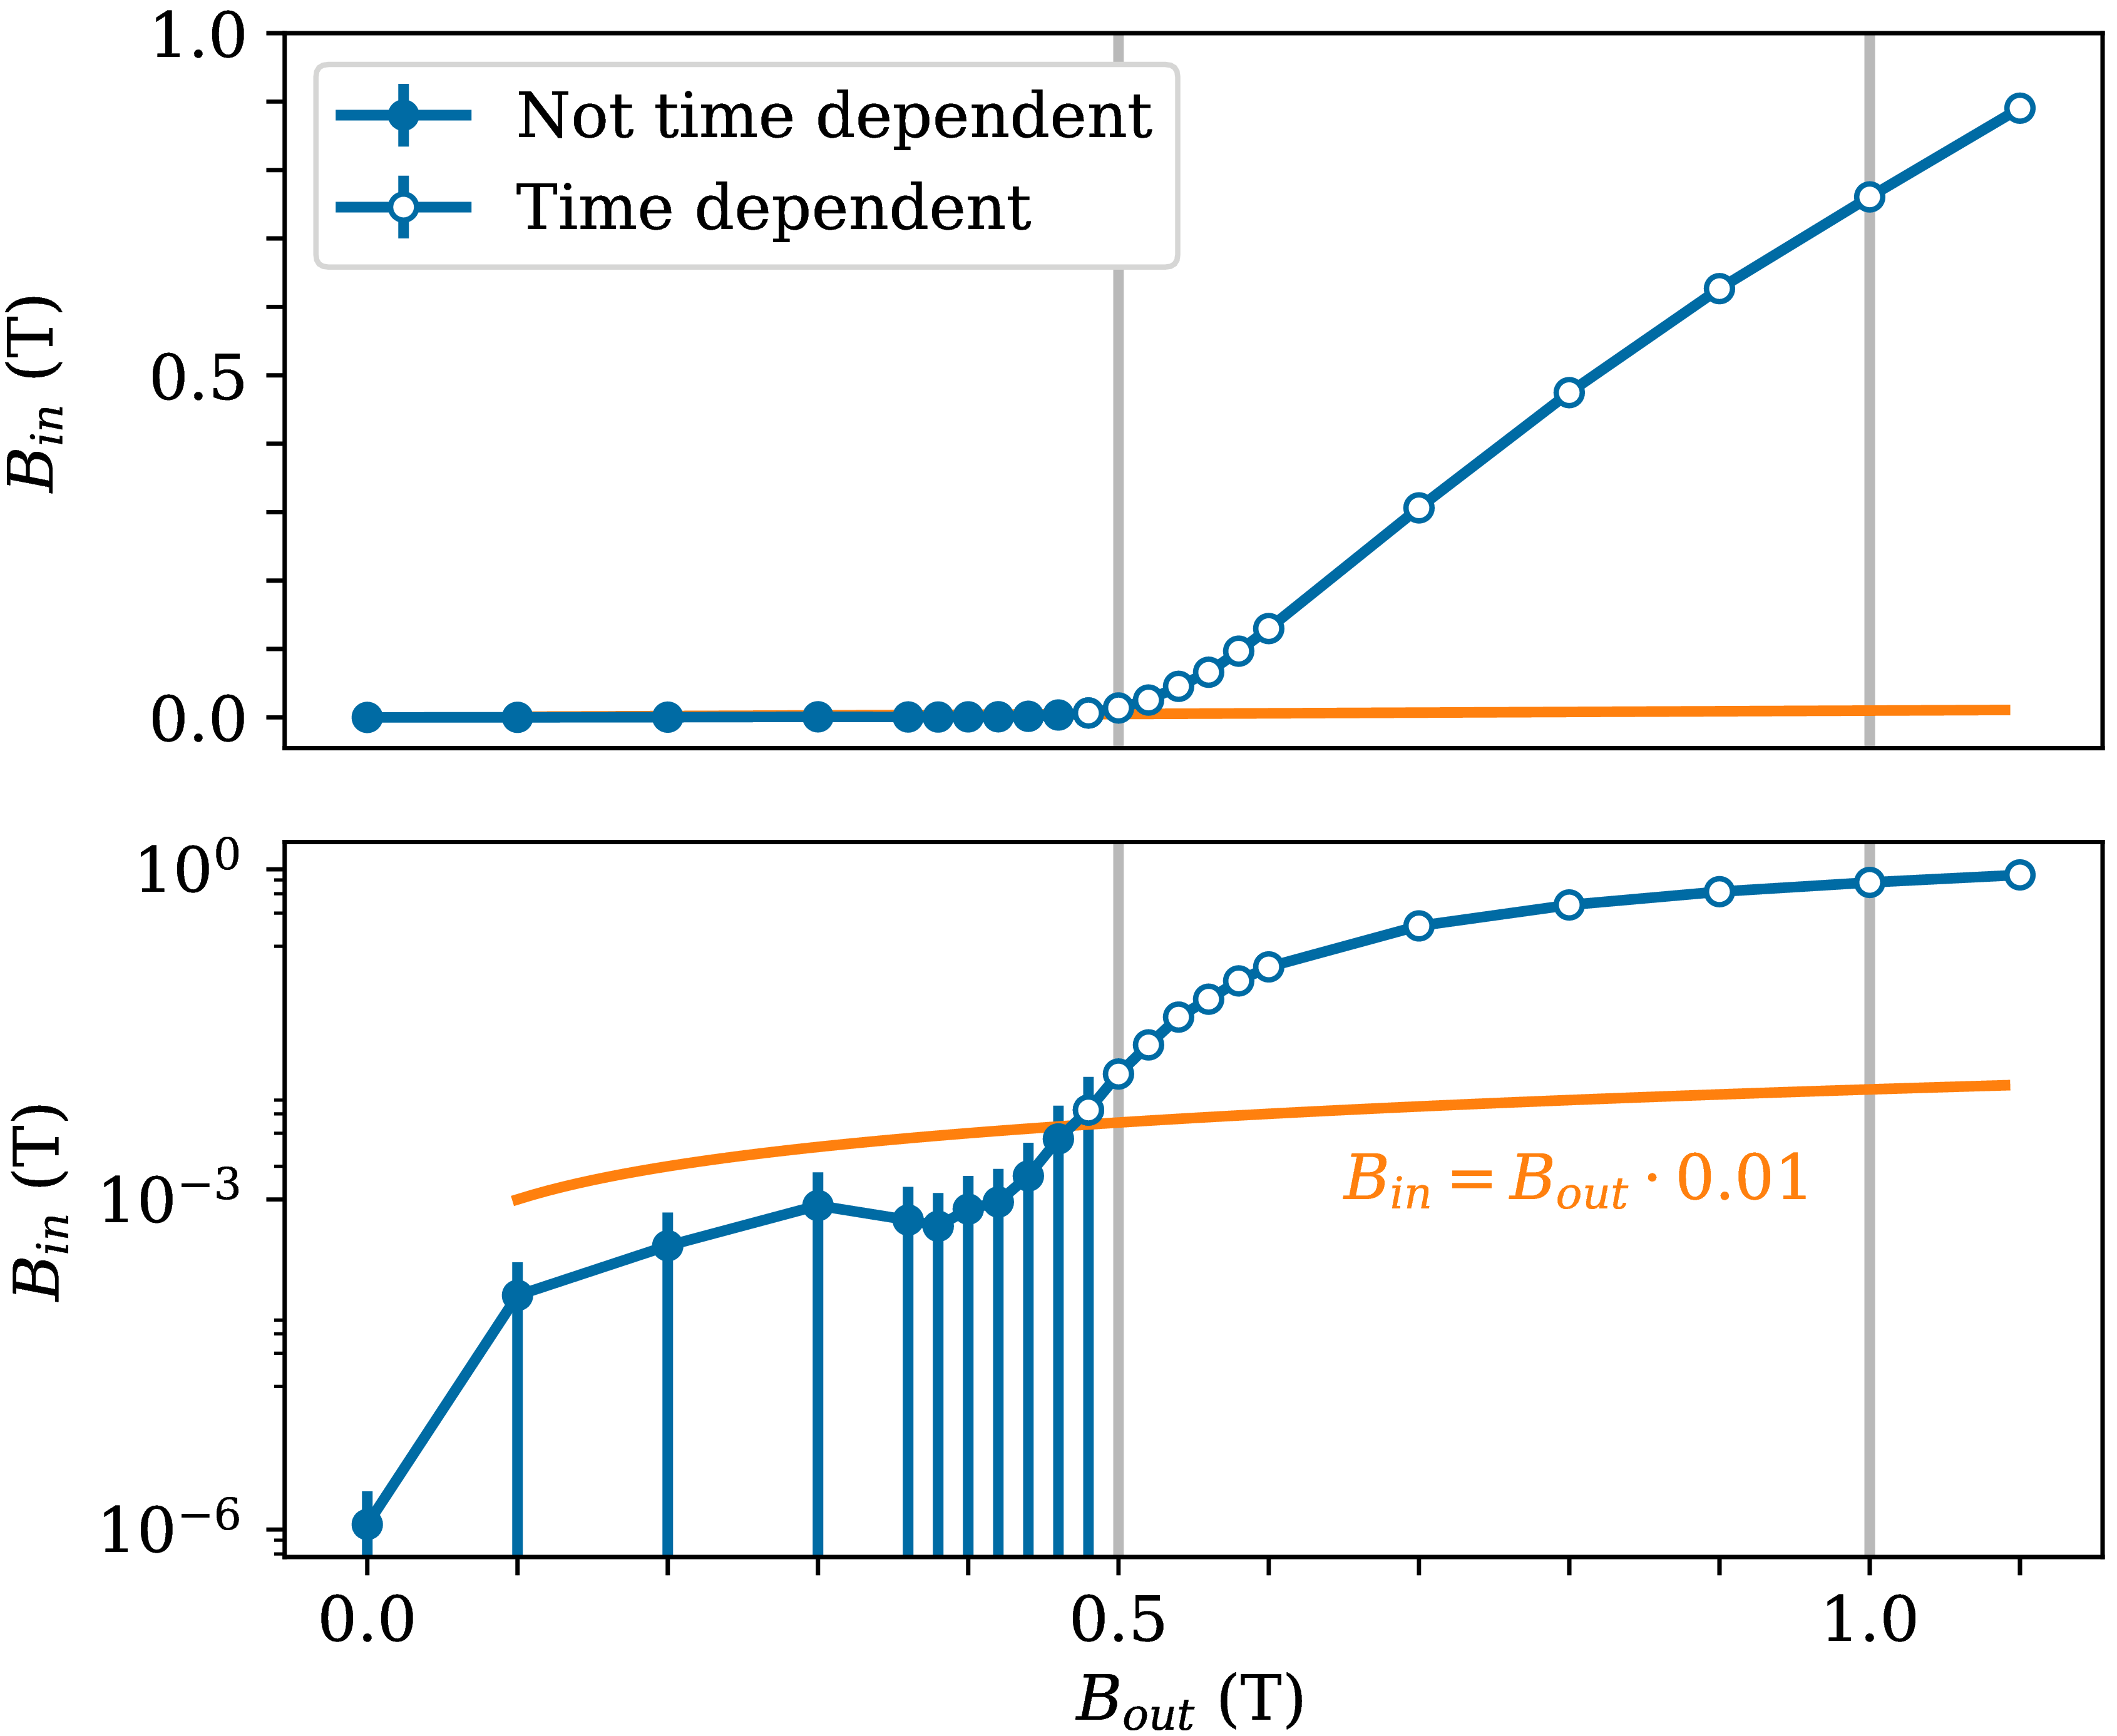
\includegraphics[width=1.0\linewidth]{shielding_mri_45layer_linlog.png}
\captionof{figure}{Measurement of shielding of the 45-layer prototype at ANL's 4-Tesla Magnet Facility.}
\end{center}
\end{multicols}


}

%----------------------------------------------------------------------------------------
%	Radiative Corrections using RADGEN
%----------------------------------------------------------------------------------------

%\headerbox{Pythia Analysis}{name=results,column=2,span=2,row=0}{
\headerbox{Experiments on the Road}{name=results,column=3,row=0}{

During the course of our experiments, we sometimes needed to travel in order to use specialized equipment. In particular, we made use of the Tandem Van de Graaff Facility at Brookhaven National Lab and the 4-Tesla Magnet Facility at Argonne National Lab.

\begin{center}
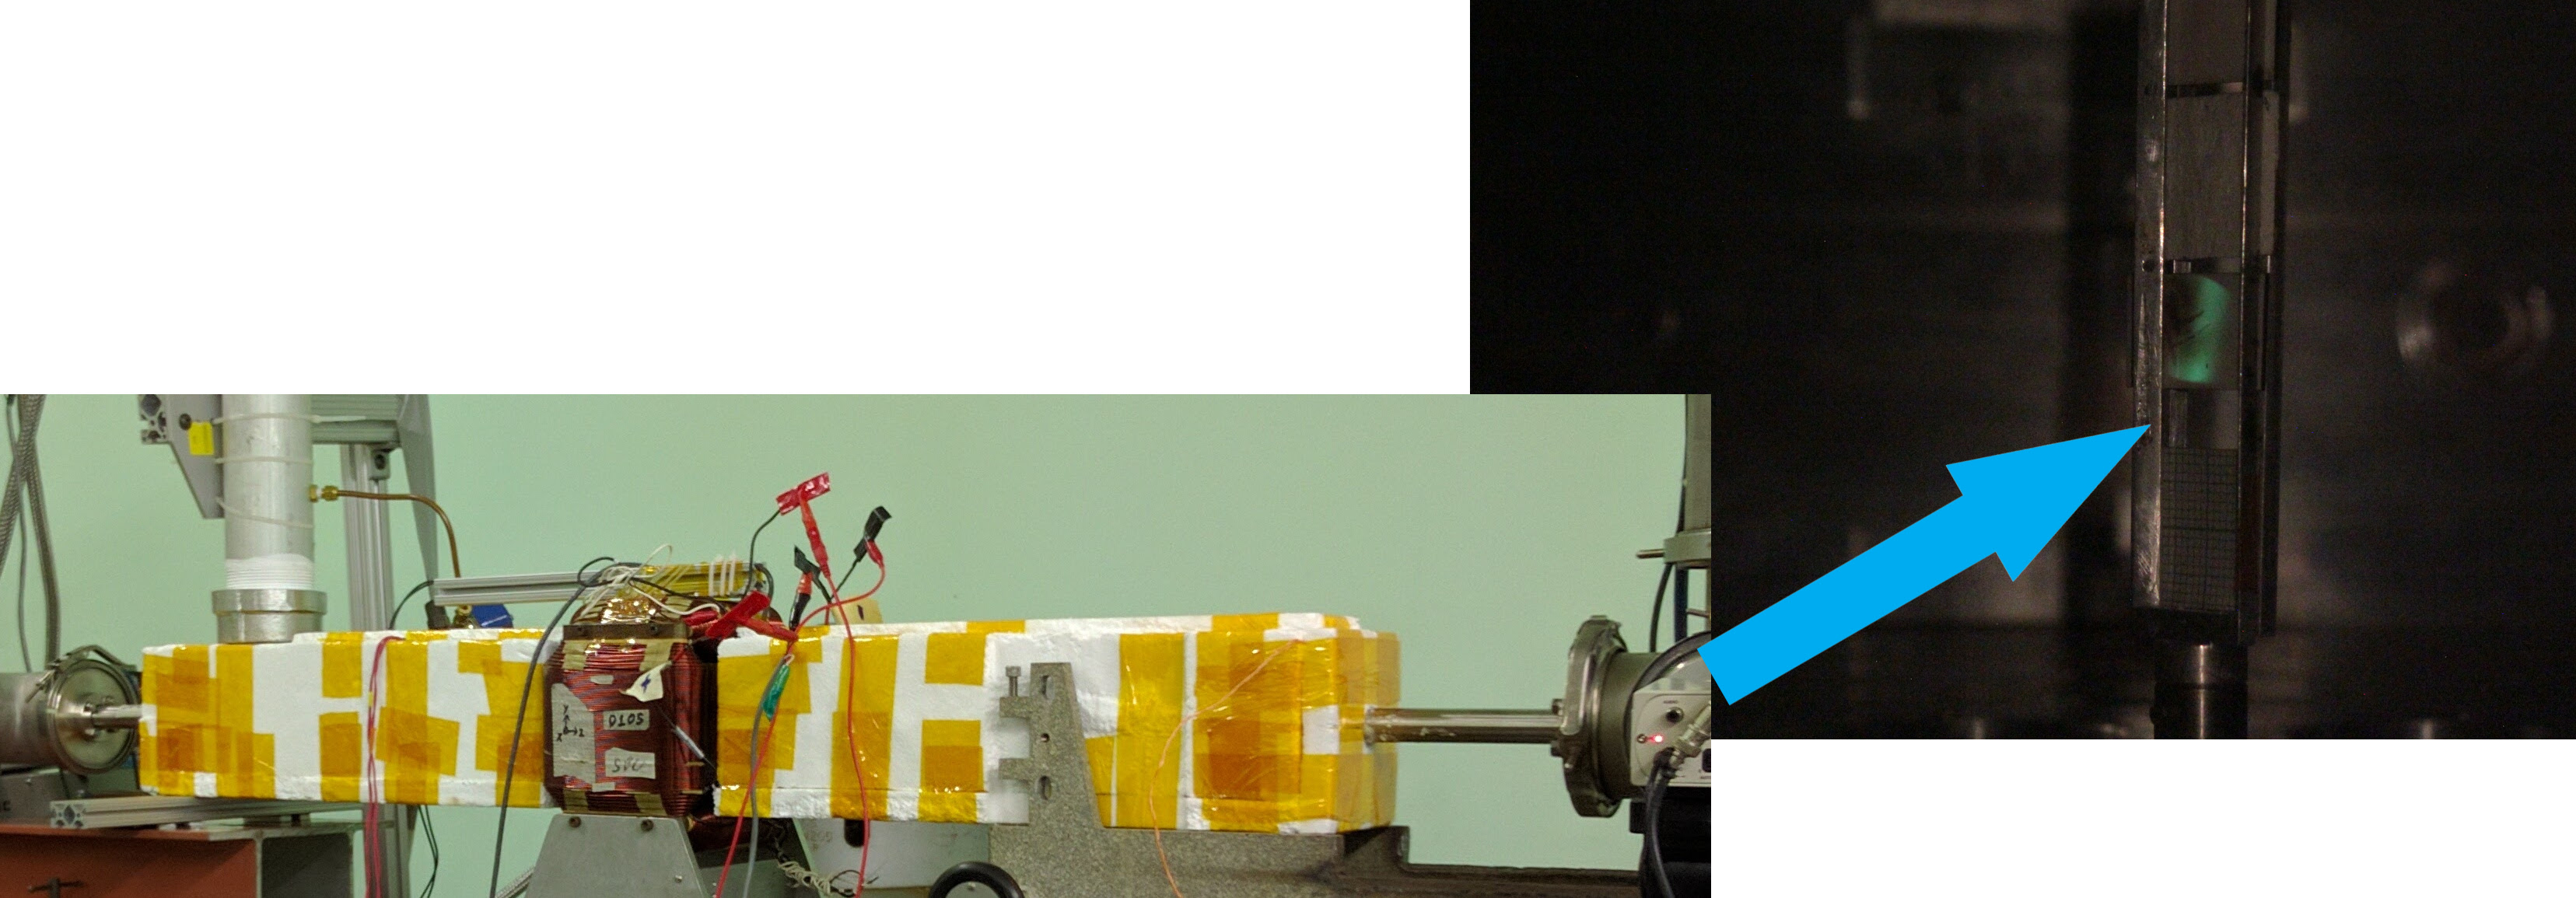
\includegraphics[width=1.0\linewidth]{bnl_beam.jpg}
\captionof{figure}{Lithium beam test at the BNL Tandem Van de Graaff.}
\end{center}

At BNL, we measured the deflection of a beam of Lithium-7 ions as they through a 1 meter long superconducting shield, which consisted of 2-layers of YBCO tape wrapped around a section of stainless steel beam pipe.

\begin{center}
\includegraphics[width=0.7\linewidth]{ANL-Pic_crop.JPG}
\captionof{figure}{Measuring magnetic field cloaking at Argonne National Lab}
\end{center}

At ANL, we measured shielding and cloaking of a 4.5-inch long, 45-layer prototype up to a field of $1.2~T$. Travel arrangements and accommodations for Argonne National Lab were handled through the university, at no cost to students.

}

%----------------------------------------------------------------------------------------
%	References
%----------------------------------------------------------------------------------------

%\headerbox{Contact Information}{name=contact,column=3,aligned=references,above=bottom}{ % This block is as tall as the references block
\headerbox{References}{name=contact,column=3,below=results,above=bottom}{ % This block is as tall as the references block
\begin{tiny}

Accardi, A., et al., \textit{Electron Ion Collider: The Next QCD Frontier} arXiv:1212.1701v3(2014)
\smallbreak
PHENIX Collaboration, \textit{Concept for an Electron Ion Collider (EIC) detector built around the BaBar solenoid} arXiv:1402.1209v1(2014)

\end{tiny}
}

%----------------------------------------------------------------------------------------
%	Further Research
%----------------------------------------------------------------------------------------

%\headerbox{Geant4 Analysis}{name=conclusion,column=2,span=2,row=0,below=results,above=references}{
%\headerbox{Further Research}{name=conclusion,column=3,row=0,below=results}{

%\begin{multicols}{2}

%\end{multicols}
%}


%----------------------------------------------------------------------------------------
%	Geant4 Simulation
%----------------------------------------------------------------------------------------

\headerbox{Magnetic Field Cloaking}{name=results2,column=1,span=2,below=introduction,bottomaligned=contact}{ % This block's bottom aligns with the bottom of the conclusion block
\begin{multicols}{2}
\begin{center}
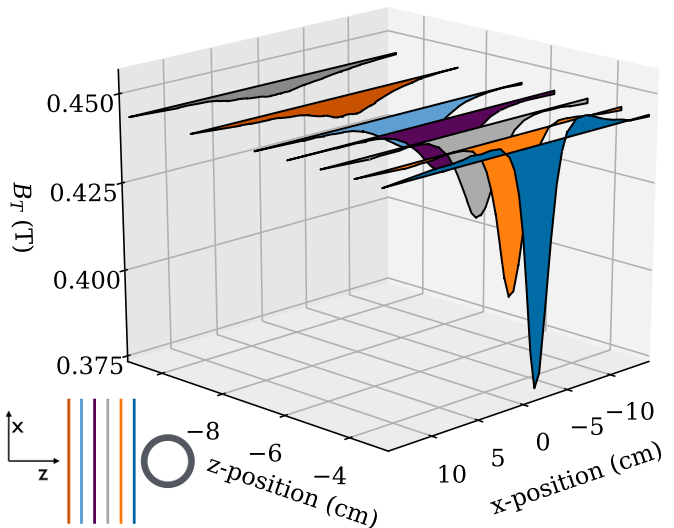
\includegraphics[width=1.0\linewidth]{NoCloak_edit.png}
\captionof{figure}{MRI Field with Superconductor Shield}
\end{center}
\begin{center}
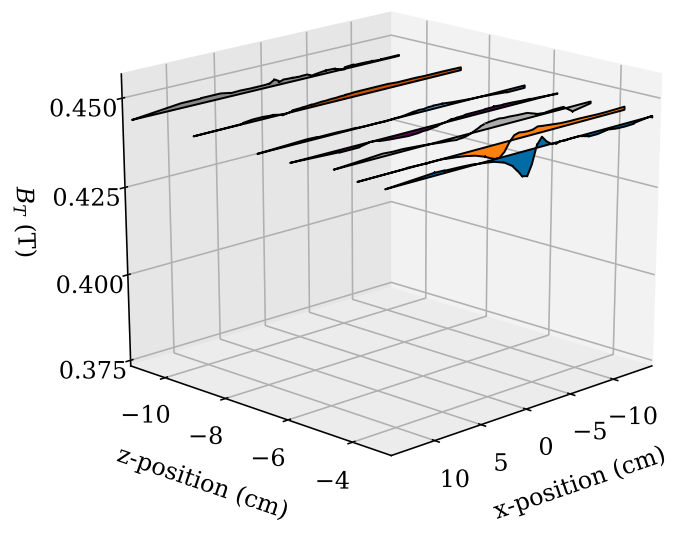
\includegraphics[width=0.95\linewidth]{WithCloak.png}
\captionof{figure}{MRI Field with Magnetic Field Cloak}
\end{center}
\end{multicols}


}

%----------------------------------------------------------------------------------------

\end{poster}

\end{document}